\chapter{Maintenance}
\section{E-beam evaporator maintenance}
\begin{figure}[H]
	\centering
	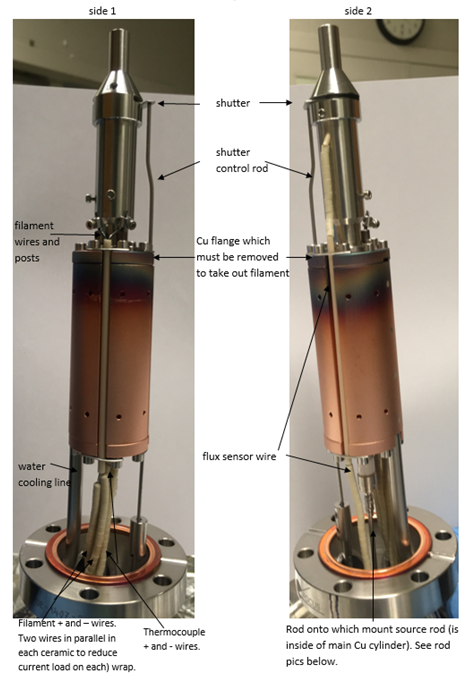
\includegraphics[width=0.6\textwidth]{W-evaporator.png}  %set figures width to text width
	\caption{Tungsten evaporator components}
	\label{fig:W-evaporator}
\end{figure}
\subsection{Filament Replacement}
This is described in detail in the e-beam manual. Follow everything except we have changed the design of how the filament loops around the posts to make the spot-welding job easier. We add two tiny loops around each post which help hold the filament in place while spot welding. It is still quite difficult to attach; in the past we always asked Reza for help.
\begin{figure}[H]
\begin{minipage}[b]{0.33\linewidth}
	\centering
	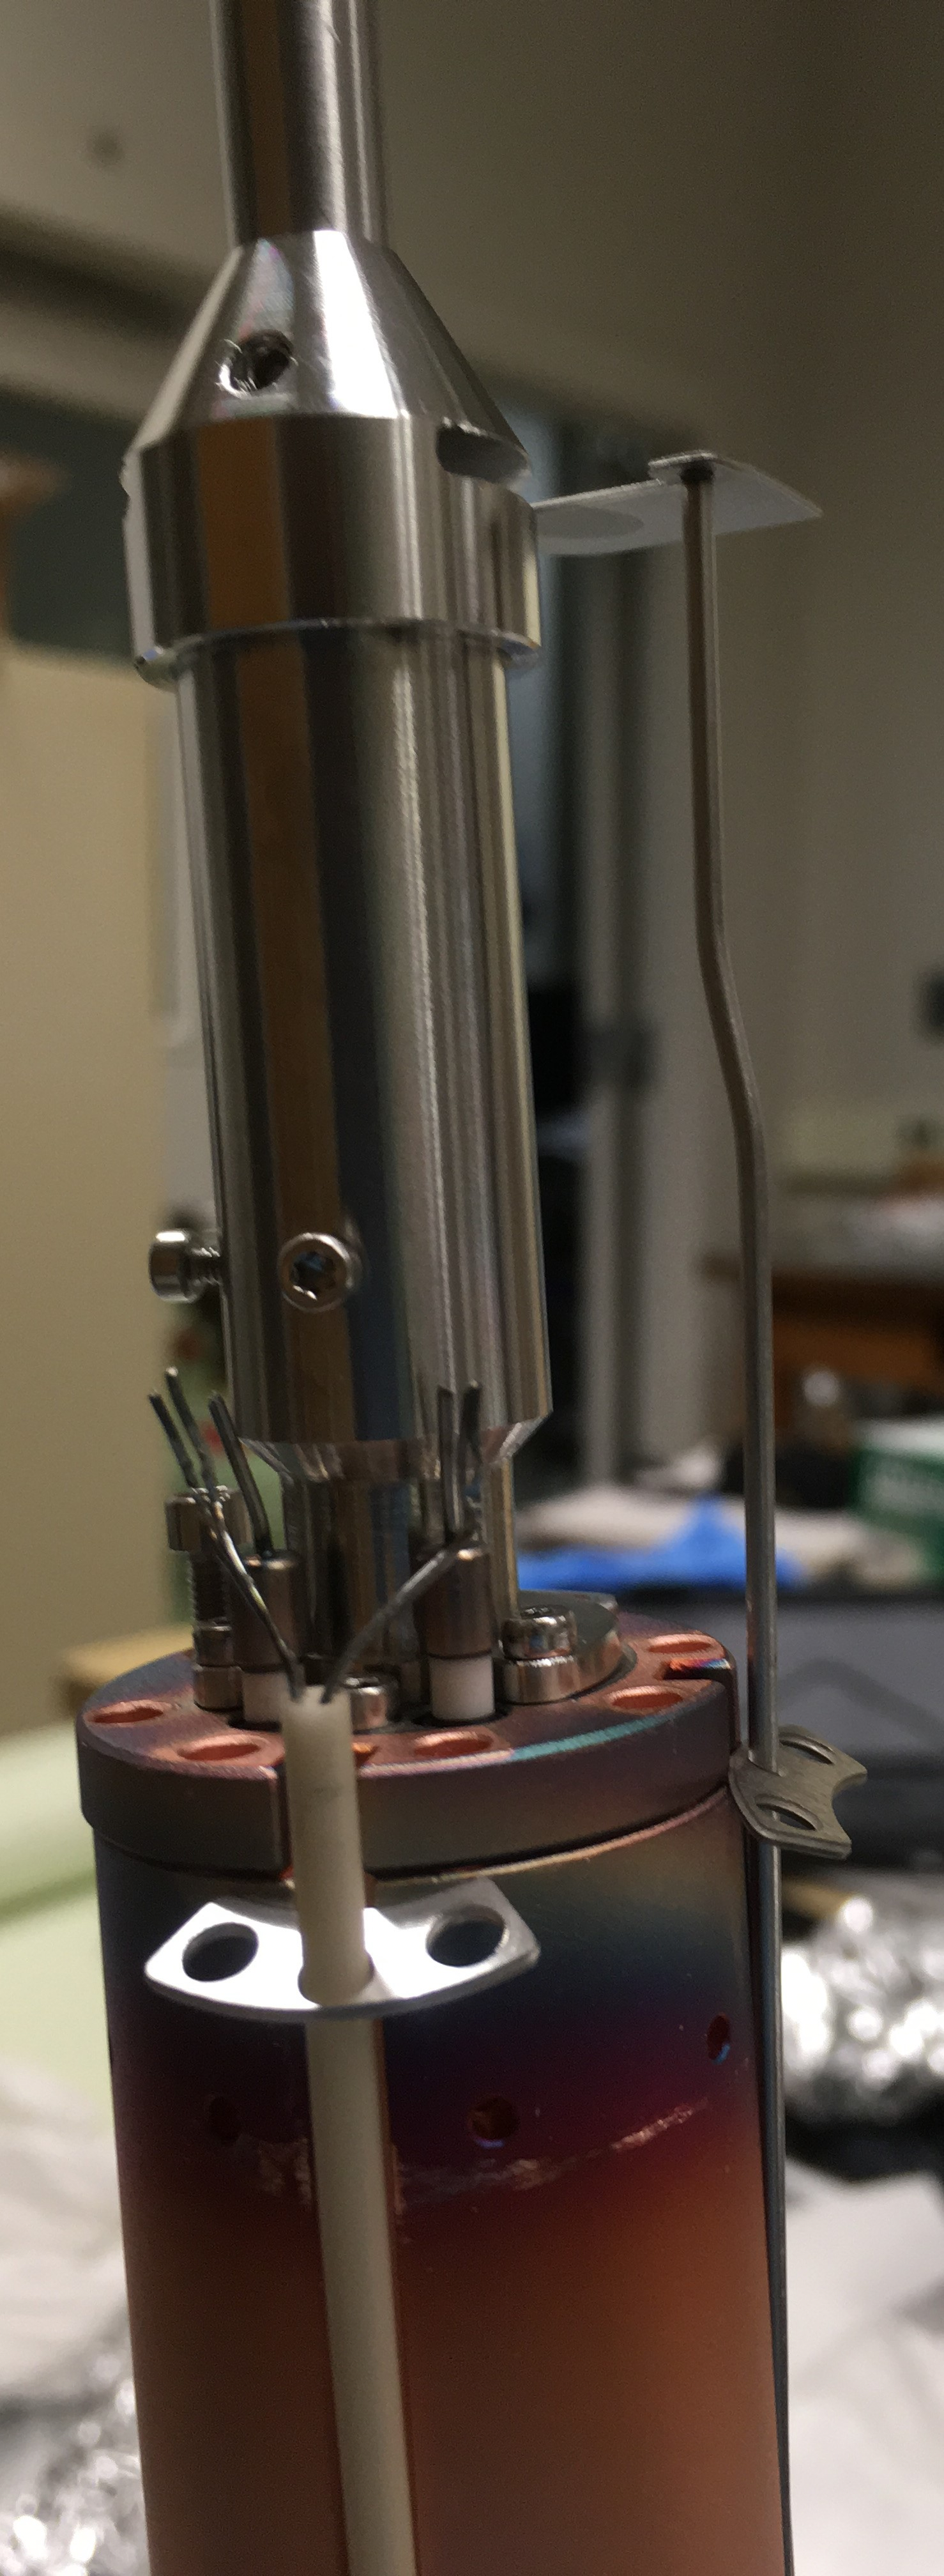
\includegraphics[width=0.5\textwidth]{partially_dissasembled.jpg}
\end{minipage}\hfill
\begin{minipage}[b]{0.33\linewidth}
	\centering
	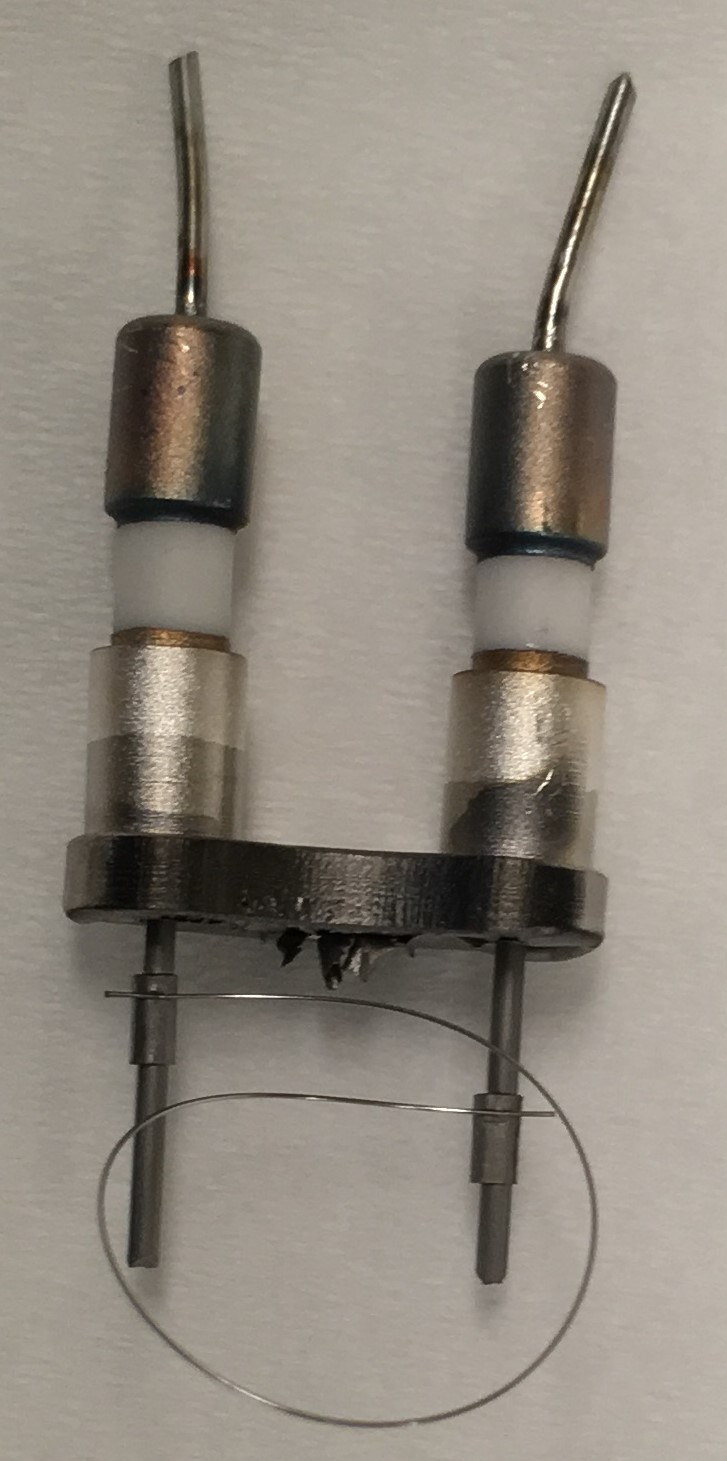
\includegraphics[width=0.4\textwidth]{filament.jpg}  %set figures width to text width
\end{minipage}\hfill
\begin{minipage}[b]{0.33\linewidth}
	\centering
	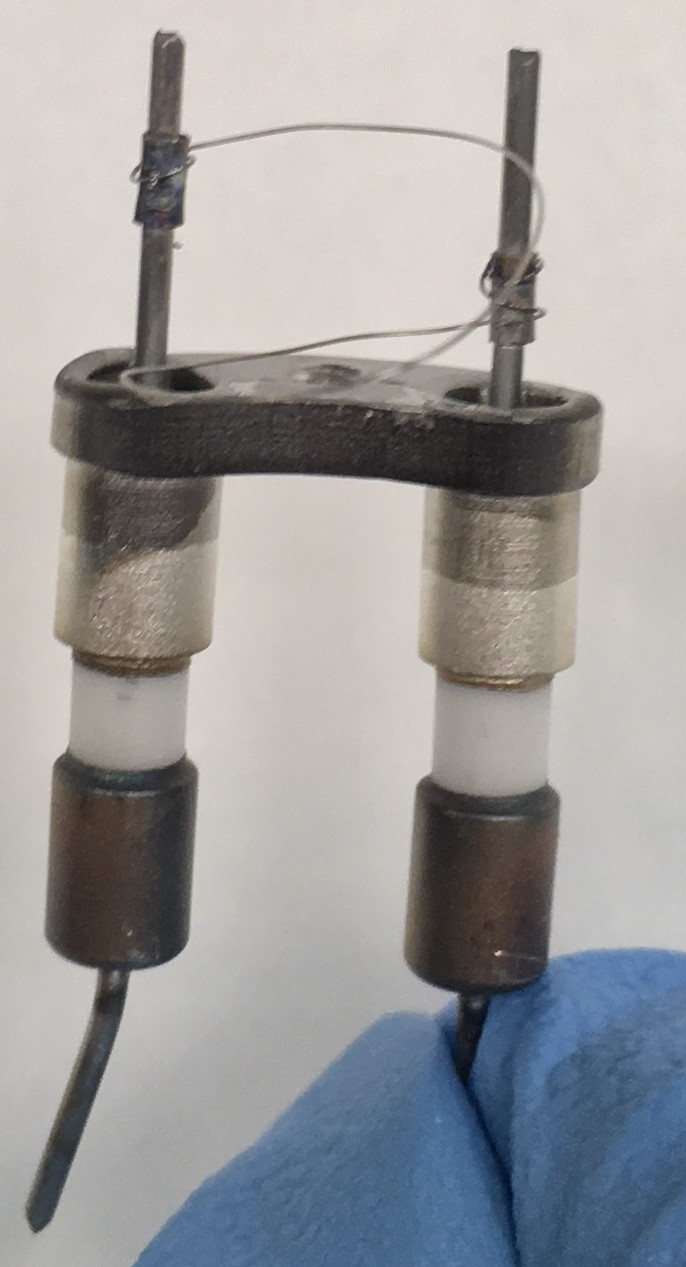
\includegraphics[width=0.4\textwidth]{filament_new_design.jpg}  %set figures width to text width
\end{minipage}\hfill
	\caption{Left: partially disassembled e-beam evaporator. Middle: Original attached e-beam filament. Right: Re-designed filament attachment.}
	\label{fig:filament}
\end{figure}

\subsection{Replenishing the source material}
\subsubsection*{Tungsten rod}
The source rod (our W rod was ~40mm in length and 1.3mm diameter) is mounted at the end of the metal rod which gets inserted into center of the evaporator. Source rod is inserted ~5mm into hole and held in place with 2 screws. When inserting and removing this rod setup must be careful to not hit the walls of evaporator so nothing gets bent. After using W rod for several months, we can clearly see the result. At the tip is small ball of W formed ($1$mm diameter, this is in contrast with the 2-3mm diameter ball that the manufacturer says will form). Also a little lower can see significantly thinner diameter of rod. This happened when rod was inserted too close to the filament and electrons were bombarding the side of the rod instead of tip.  To move source rod closer/further from filament the screw gauge outside of evaporator is moved which moves a bevel on which end this whole rod setup below is attached. The whole setup seen below moves as one piece.

\begin{figure}[H]
	\centering
	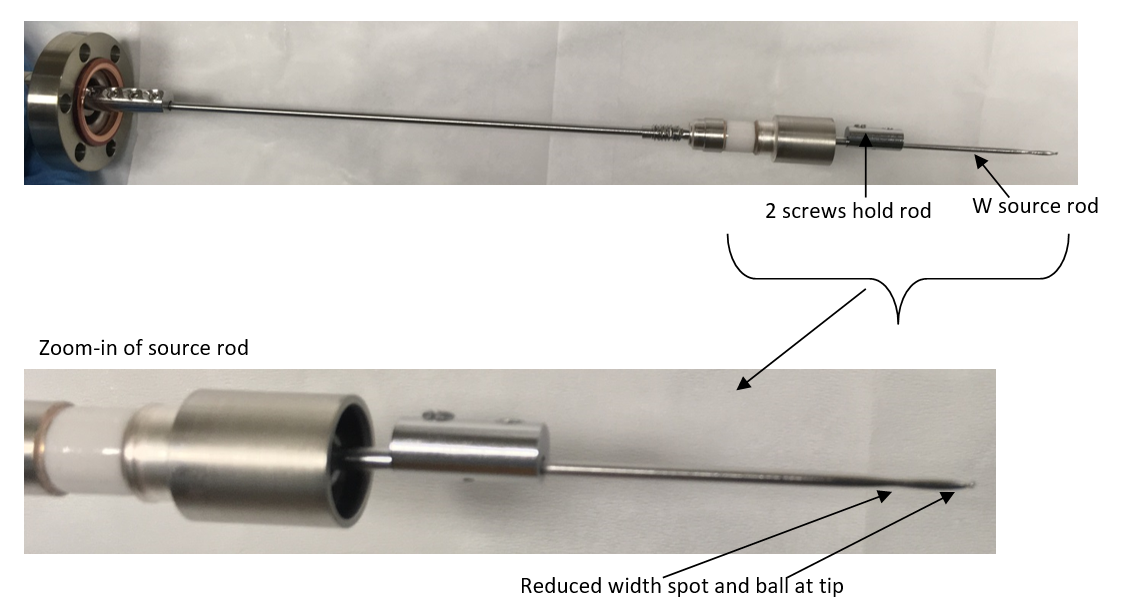
\includegraphics[width=1\textwidth]{W-rod-pics.png}  %set figures width to text width
	\caption{Tungsten rod setup}
	\label{fig:W-evaporator}
\end{figure}


\subsubsection*{Tin pellets}
Fill the crucible about $1/3$ full with pellets. This is to ensure that pellets don't fall out when slightly tilt evaporator as needed to insert it back into MBE port. Also ensures that no liquid Sn flows out of crucible. \textbf{Do not significantly tilt the evaporator or lay it down if it has source pellets in it!}.
 
\section{Removing a dropped sample}
Taking out a dropped sample (as done on 10/27/16)
\begin{enumerate}
\item	Get the mirror kit from the machine shop. Use the straight, extendable rod and the larger square mirror.  The connections of mirror to rod and spring loaded (push back at rod end, insert mirror connection and release). Wipe rod and mirror with acetone and IPA, then wrap rod and back side of mirror with foil. 
\item	Open the large port on the side of the MBE (this port’s face is vertical). Put the old gasket back and hold it in place by wrapping some foil around parts of it and the outer parts of port flange. 
\item	Open the medium sized port on the bottom (closest to water cooling manifold wall) of MBE. 
\item	Make sure QCM is all the way retracted and z manipulator all the way up. Turn on the 2 LED lights at the viewports. 
\item	Now have 1 person carefully move the mirror into the large side port. Other person lays on the floor and looks up through the bottom port at the mirror. Person with mirror moves mirror around so other person can see the bottom of the chamber and try to find the sample.
\item	Once see the sample, procedure to take it out depends on where it is:
\begin{enumerate}
\item	If sample is in one of the bottom ports, then it is easiest. Simply open that port and sample will fall out.
\item	If sample is on the chamber floor, and there is a large enough port nearby (i.e. the one you are looking through at the bottom), then can take out the sample by hand. Must wear clean gloves and either wrap arm with clean foil or wear special shield (Andrew has), like cleanroom shield up to the elbow. It is easier to take out sample by hand than with some tool, since hand can feel the sample and grab it. 
\item	If sample is near a port that is too small to fit hand into or not near a port/ evaporator, then need to use a tool to move sample to a port and drop it into there. The other rod from the mirror kit (the flexible rod) can serve as the tool. Wipe this with acetone and IPA and wrap with foil. Then bend in the necessary shape and try to move the sample to a port by inserting the tool through one of the other opened port. It is useful to also make the mirror stay in place (easiest way is to simply put bunch of foil at exit point of the side port where mirror is, so mirror is resting on the foil) and use it to see what you are doing. Once have pushed the sample into a port, just open that port to take it out. 
Remember to change gaskets on all ports you have opened before re-tighten them for the final time before bakeout. These ports are to the main MBE system, so we do not want to re-use the gaskets since a leak is risky.
\end{enumerate}
\end{enumerate}
\section{Degassing a new Ta crucible}
Degassing New Ta crucible:
A new crucible must be degassed before using. Crucible is installed without any source material into evaporator. Then evaporator is run which heats up the crucible and cleans it from dirt/impurities. The parameters values refer to those observed when we degassed a crucible for first time in Sn evaporator on 9/23/16.
\begin{enumerate}
\item	Turn on water cooling (can do this day before to be able to check for leaks and save time).
\item	Connect liquid N2 hose. Make sure that using a full dewer (it is very inconvenient if L N2 runs out mid-process). Start filling cryostat. It will need to be periodically refilled during the process.
\item	Turn on evaporator controller. If it doesn’t turn on, check the MBE interlock screen on touch screen to make sure that “activate devices” is selected.
\item	Shutter can be kept either open or closed. We usually keep it closed b/c if keep shutter open the liquid N2 is used up much more since more heat gets transferred to the MBE chamber.
\item	Since evaporator filament was exposed to air when filled the crucible, first need to degas the filament: Keeping HV (high voltage) off (therefore there will be no e-beam hitting the crucible), gradually ramp up FIL (filament current) to 2.0A in increments of 0.1-0.2A. Will see jumps in FLUX (flux current) as filament degasses. Wait to make sure FLUX is decreasing before further increasing FIL.
\item	Now can degas the crucible. Tune FIL down to 0. Gradually ramp up HV to 2000V. Then gradually increase FIL until either there is a rise in MBE chamber pressure or EMIS reaches 5mA. When we did it, a jump in pressure occurred when FIL reached ~1.0A at which EMIS was still 0mA. Wait for pressure to stabilize before continuing to increase FIL. Pressure might not go back down to initial levels, but as long as it stays constant for some time, can keep going. Keep pressure under ~1e-7 during entire degassing procedure. 
\item	Keep increasing FIL using small (i.e. 0.05) steps if have pressure instability. When FIL reaches 1.5A, EMIS increases from 0 to 0.1mA. Flux rose to $>1$nA when EMIS reached 0.2mA and FIL=1.55A. Flux will rise to higher values when increase FIL more, but generally should then decrease since once dirt has been removed from surface, there should not be more dirt coming off. Flux was 2.75nA when EMIS reached 1mA. Note that there will likely be a quite significant delay (up to several minutes) between turning the current dial and EMIS increasing especially during initial stages of degassing. We think this is due to that there is an initial degassing of the filament itself, after which it is more efficiently emitting electrons which results in the EMIS rise. Also we notice that after a while the FIL decreases a little, again indicating that it is being cleaned and improving as we proceed.
\item	Controller switches to EMIS control (using a setpoint and feedback) when EMIS reaches 1.5mA.  Reaching to 5mA will take some time since there is a lot of initial degassing occurring. At EMIS = 2.2mA, MBE pressure rose to mid $10^{-8}$ from starting pressure of low $10^{-9}$s. After reach 10mA EMIS, can increase EMIS much faster since no longer have such large pressure jumps. Continue increasing EMIS in 5mA increments (5, 10, 15mA) and record all observed parameters right when reach that specific EMIS current and later after the parameters have stabilized. Since the flux generally continues to slowly decrease over a long time, we defined “stabilized” as 3 minutes after initially increasing to certain EMIS value and all other parameters are stable.
\item	The goal was to increase EMIS up to the maximum possible 150mA which with the 2000V HV would provide 300W of power to the crucible. This was the recommendation that the manufacturer gave us for degassing the crucible. However, after reaching 115mA, we observed very high flux current, reaching $\mu A$ level and not decreasing. We were concerned about evaporating the crucible itself (fortunately when we took out evaporator, we confirmed that no damage was done to the crucible), since contaminants should result in a decreasing flux after the initial increase. Even when decreasing EMIS to 100mA, we still observed a gradually increasing FLUX of ~$\mu A$.  Therefore we stopped degassing at this point.
\item	Gradually tune current down to zero, then ramp voltage down. Turn off evaporator. Need to wait for the crucible to cool before vent the system and take out evaporator to fill it with source material. Keep the water cooling running while the evaporator cools. Best to keep it running overnight.
\end{enumerate}
